% Software Development for Mobile Devices
\documentclass[11pt,english,numbers=endperiod,parskip=half]{scrartcl}

\usepackage{color}
\usepackage{graphicx}
\usepackage{minted}
\usepackage{fancyhdr}
\usepackage{pdflscape}
\usepackage{listings}
\usepackage{pifont}

\newcommand{\cmark}{\ding{51}}

\pagestyle{fancy}

\rhead{Daniel Parker - 971328X}
\lhead{COS30017 - Software Development for Mobile Devices}

\title{Portfolio Report}
\subtitle{COS30017 - Software Development for Mobile Devices}
\author{Daniel Parker 971328X}

\date{\today}

\begin{document}
\maketitle
\thispagestyle{empty}

\section{Overview}

\section{Evidence}
\textit{\textbf{-} = in progress}
  \begin{table}[H]
    \begin{tabular}{|l|c|}
      \hline
      Assessment & Completed \\
      \hline
      Core Assignments (for Pass) & \cmark \\
      \hline
      Extension Tasks (for Credit) & \cmark \\
      \hline
      Custom Application (for Distinction) & \textbf{-} \\
      \hline
      Research Report (for HD) & \textbf{-} \\
      \hline
    \end{tabular}
  \end{table}
  Project brief has been submitted for custom application and I also intend on
  completing the HD research report as well.
\section{Reflection}
  \subsection{Concept Map}
    \begin{figure}[H]
    \centering{
      \fbox{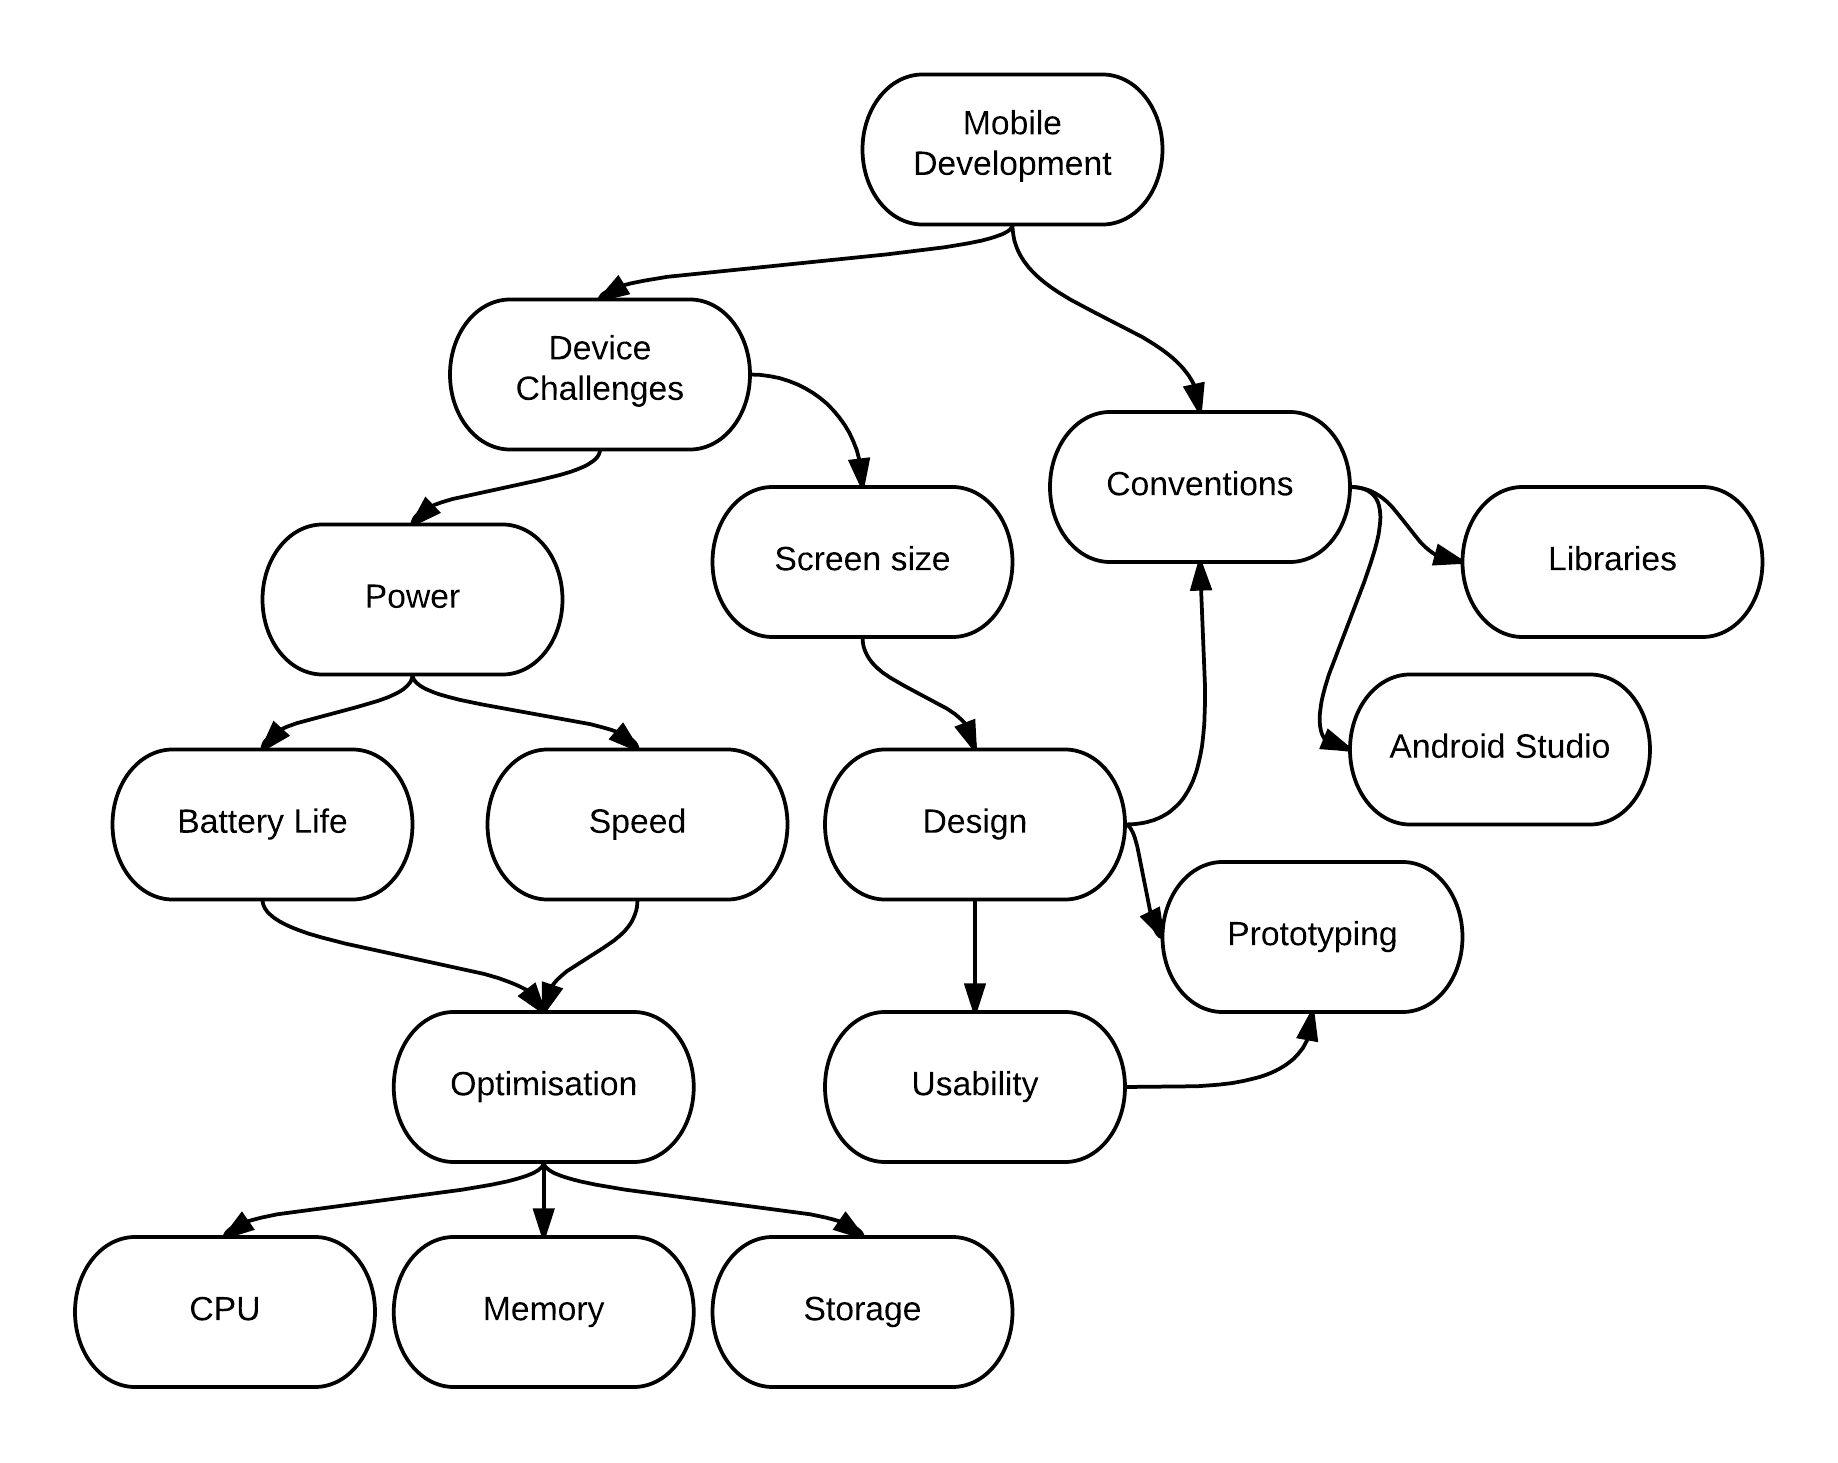
\includegraphics[width=\textwidth]{images/mind_map.png}}
    }\\
    \end{figure}
  \subsection{Mobile Application Development Process}
    The process to developing a mobile application is in a lot of ways a
    combination of web development and conventional desktop application development.
    From desktop application development comes the usual development methodologies
    such as agile, scrum etc., which are proven in providing a good and reliable
    framework for delivering applications. The web development processes that
    are also inherited by mobile development are those of iterative app design,
    user interface and usability testing, and then heavy design implementation.

    At a high level the resulting process for designing mobile applications is
    as follows:
    \begin{enumerate}
      \item{
        Ideation - Exploring the app's idea, what it will do, features etc.
      }
      \item{
        Exploration - User stories/scenarios, constraints, UI sketches and
        heuristic evaluation.
      }
      \item{
        Initial Clarification - Navigation flow, hi-fi prototype and usability
        test.
      }
      \item{
        Executable Prototype - Create prototype, validate the app.
      }
      \item{
        Iterative Development - Continue developing features, run usability
        tests and other validation methods to assist with refining.
      }
    \end{enumerate}
  \subsection{Analysis and Problem Solving Approaches}

  \subsection{Comparison and Contextual Placement}

  \subsection{Generalization}

  \subsection{Challenges in Mobile Development}
    The combining of these two different development domains creates some
    interesting challenges in mobile development. One aspect of Android
    development in particular that's accentuated heavily on is the concept of
    `Convention over Configuration', and this is apparent when using the newest
    Android integrated development environment, Android Studio. Every part of an
    Android application has it's place in the structure of the project, to the
    point where if it's not in that location, then the app may not compile
    correctly. Anything to do with layout, design, dimensions, string constants
    and much more must be placed in their respective directories and xml files
    within the `res' directory, whereas any application logic needs to go in the
    `java' directory.
  \subsection{Explorations}

\end{document}
